\documentclass[11pt, a4paper]{article}
\usepackage{graphicx} % Required for inserting images
\usepackage{listings}
\usepackage{color}

\title{A Web Based Command Line Interface for Specifying Multiway Dataflow Constraint Systems}
\author{Bo Aanes}
\date{June 2023}
\lstset{
    frame=single,
    basicstyle=\linespread{0.8}\footnotesize\ttfamily,
    keywordstyle=\color{red},
    numbers=left,
    numbersep=5pt,
    showstringspaces=false, 
    stringstyle=\color{blue},
    commentstyle=\color{gray},
    breakatwhitespace=true,
    breaklines=true,
    postbreak=\mbox{\textcolor{violet}{$\hookrightarrow$}\space},
    tabsize=4,
}

\begin{document}

\begin{titlepage}
    \centering
    \vspace*{\fill}
    {\scshape\LARGE University of Bergen\par}
    \vspace{1.5cm}
    {\huge\bfseries A Web Based Command Line Interface for Specifying Multiway Dataflow Constraint Systems\par}
    \vspace{2cm}
    {\Large\itshape Bo Victor Isak Aanes\par}
    \vfill
    {\large \today\par}
    \vspace{1cm}
    {\large INF319 Project\par}
    \vfill
\end{titlepage}
\tableofcontents
\clearpage

\section{Introduction}
\label{sec:introduction}
Graphical user interfaces (GUIs) are prevalent in most of today's technology that involves user interaction. However, developing and maintaining GUIs can still be difficult. Much of this is because as a GUI involves a larger set of state, the business logic neede in order to keep track of this state quickly becomes complex. This problem grows even bigger when we introduce dependencies between elements of the GUI. Multiway dataflow constraint systems (MDCS) is a programming model designed to let a developer specify dependencies between elements of the GUI using constraints \cite{semantics}. This is usually done declaratively and MDCS will handle all business logic related to these constraints. 

\section{Background}
\label{sec:background}
\subsection{Multiway Dataflow Constraint Systems}
\label{sec:mdcs}
A multiway dataflow constraint system consists of a set of variables and a set of constraints. A variable holds a value which can be modified, and a constraint consists of a set of methods which contain expressions that can modify a variable.

Libraries that implement MDCSs usually also handles enforcing of constraints, such that whenever a value gets updated by a user the constraint system automatically satisfies all its constraints. The main part of \textit{solving} a constraint system is achieved through what is called \textit{planning} \cite{planners}. When a variable is updated by a user, the constraints involving this variable may no longer be satisfied, that is, that the relations specified in the methods no longer hold. As such, we have to select the appropriate methods to invoke in order to enforce the given constraints, such that the constraint system is satisfied. This is what the planner does.

When a user updates a variable, they will expect that the constraint system does not overwrite that variable instantly. Because of this we do not want the planner to select a method writing to this variable, but rather a method that reads from it. I.e., we want to select the methods from the constraints that result in the least surprising outcome to the user. This is what is known as a \textit{hierarchical} planning algorithm \cite{planners}.

The hierarchical planner assigns a strength to each variable, which gets updated when a user modifies a variable. The variable with the highest strength is the one that was updated most recently, and the variable with the lowest strength was the one updated least recently. By assigning a strength to the variables, the planner can make selections on which variables to preserve by selecting the appropriate methods.

When the appropriate methods are selected, they are invoked in the topological order of the dataflow graph. This is done to ensure that all variables are updated in the correct order, such that no variable is updated before its dependencies are updated.

\subsection{HotDrink}
\label{sec:hotdrink}
HotDrink is a JavaScript library for specifying multiway dataflow constraint systems \cite{hotdrink}. It provides both an API and a DSL for this purpose. Variables can be declared along with constraints between these, which in turn can be bound to specific HTML-elements. The constraints themselves contain \textit{methods} which can hold expressions or JavaScript functions that return values which are written to specified variables. In Listing \ref{lst:currencyhotdrink}, we can see how we can use HotDrink's API and DSL to define a constraint system to perform currency conversion between EUR and NOK.

\begin{lstlisting}[language=java, caption={Currency conversion in HotDrink.}, label={lst:currencyhotdrink}]
const constraintSystem = new ConstraintSystem();

const component = component`
    var exchangeRate = 10;
    var eur = 0;
    var nok = 0;

    constraint {
        eurToNok(eur, exchangeRate -> nok) = eur * exchangeRate;
        nokToEur(nok, exchangeRate -> eur) = nok / exchangeRate;
    }
`;

constraintSystem.addComponent(component);
constraintSystem.update();
\end{lstlisting}

We first define a constraint system using the \texttt{ConstraintSystem} class. We then define a component using the \texttt{component} template literal, which contains specifications for a currency conversion using HotDrink's DSL. Here we define variables and a constraint containing two methods: one for converting EUR to NOK, and one for converting NOK to EUR. After specifying our component, we add this component to the constraint system and call \texttt{constraintSystem.update()} to enforce the constraint.

The variables defined in the constraint system in Listing \ref{lst:currencyhotdrink} can be bound to elements in the document object model (DOM), e.g., two input fields. When the user changes one of these input fields, the other one's value will be updated to the correct value determined by the constraint system.

\subsection{Structure Manipulation}
\label{sec:structuremanipulation}
\textit{WarmDrink} is a domain specific language (DSL) for defining relation between components in constraint systems \cite{warmdrink}. This allows for defining what we call \textit{intercalating constraints} which can manipulate values between elements in structures such as lists or trees. An example of this could be a multi-city flight itinerary \cite{warmdrink}. Let us say the first flight is at 15th of June, then the next flight can be no earlier than 15th of June as well. This relation can be introduced as an intercalating constraint between all flights in flight itinerary. The date of each flight must be equal to or greater than the preceding flight's date. If one of the flight's date gets updated, then so must all the succeeding flights as well.

\subsection{React}
\label{sec:react}
React is a JavaScript library for building user interfaces \cite{react}. It is based on the concept of components, which are reusable pieces of code that can be composed together to build complex user interfaces. React components are written in JavaScript, and can be written using either a class-based or a functional approach. In Listing \ref{lst:reactcomponent}, we can see an example of a React component written using the functional approach. Notice how the \texttt{return}-function contains HTML-like syntax. This is known as JSX (or JavaScript XML), which is an extension of JavaScript's syntax that allows for using HTML directly in you JavaScript files. React then transpiles the code into regular JavaScript, which can be run in a web browser.

\begin{lstlisting}[language=java, caption={A React component written using the functional approach.}, label={lst:reactcomponent}]
function MyComponent(props) {
    return (
        <div>
            <h1>{props.title}</h1>
            <p>{props.text}</p>
        </div>
    );
}
\end{lstlisting}

React components can be rendered to the DOM using the \texttt{ReactDOM.render} method. This method takes a React component and a DOM element as arguments, and renders the component to the DOM element. In Listing \ref{lst:reactrender}, we can see how we can render the component from Listing \ref{lst:reactcomponent} to the DOM. Notice how we pass \textit{props} from the parent component down to the child component within the JSX.

\begin{lstlisting}[language=java, caption={Rendering a React component to the DOM.}, label={lst:reactrender}]
ReactDOM.render(
    <MyComponent title="Hello, world!" text="This is my first React component." />,
    document.getElementById('root')
);
\end{lstlisting}

\subsection{Web Application Programming Interfaces}
\label{sec:apis}
An application programming interface (API) is a set of rules and protocols for building software applications. It defines how different software components can interact with each other. This can for example be between a frontend web application and a backend database. This is known as a Web API, or an HTTP API.

A web server can provide \textit{endpoints} for a client to send requests to. These endpoints are URLs that the client can send HTTP requests to, and the server will respond with a HTTP response. The client can send different types of requests, such as GET, POST, PUT, and DELETE. These requests are used to retrieve, create, update, and delete data from the server, respectively. The server can then respond with different types of responses, such as 200 OK, 201 Created, 400 Bad Request, and 404 Not Found. These responses are used to indicate whether the request was successful or not, and can also contain data.

\subsection{Haskell}
\label{sec:haskell}
Haskell is a purely functional programming language first released in 1990 \cite{haskell}. It is a statically typed general purpose language which uses lazy evaluation and type inference. Lazy evaluation is a technique where the compiler does not evaluate expressions until they are needed. And type inference is a feature in the compiler which can infer the types of expressions without them having to be explicitly annotated in the actual code..

Haskell also provide a powerful type system, which allows for the creation of custom types and type classes. Type classes are similar to interfaces in object-oriented programming languages, and can be used to define functions that can be used on different types. For example, the \texttt{Show} type class defines a function \texttt{show} which can be used to convert a value to a string. While the \texttt{Eq} type class is used for determining equality between values.

Data types in Haskell can be considered algebraic data types. They can be either \textit{product types} or \textit{sum types}. Product types are types that contain multiple values, such as tuples and records. Sum types are types that can be one of multiple types, such as the \texttt{Maybe} type. The \texttt{Maybe} type can either be \texttt{Just a} or \texttt{Nothing}, where \texttt{a} is a type variable. This type is used to represent values that may or may not be present, such as the result of a database query.

\newpage

\section{Frontend}
\label{sec:frontend}
The frontend part of our CLI tool is written in TypeScript \cite{typescript} with React as our frontend library of choice.The main component \texttt{App} is the root component of our frontend and embodies everyhting the user sees and interacts with. The user is presented with a split screen consisting of a two main components: the view of the constraint system, and the terminal, see Figure \ref{fig:view}.

\begin{figure}[h]
    \centering
    \makebox[\textwidth][c]{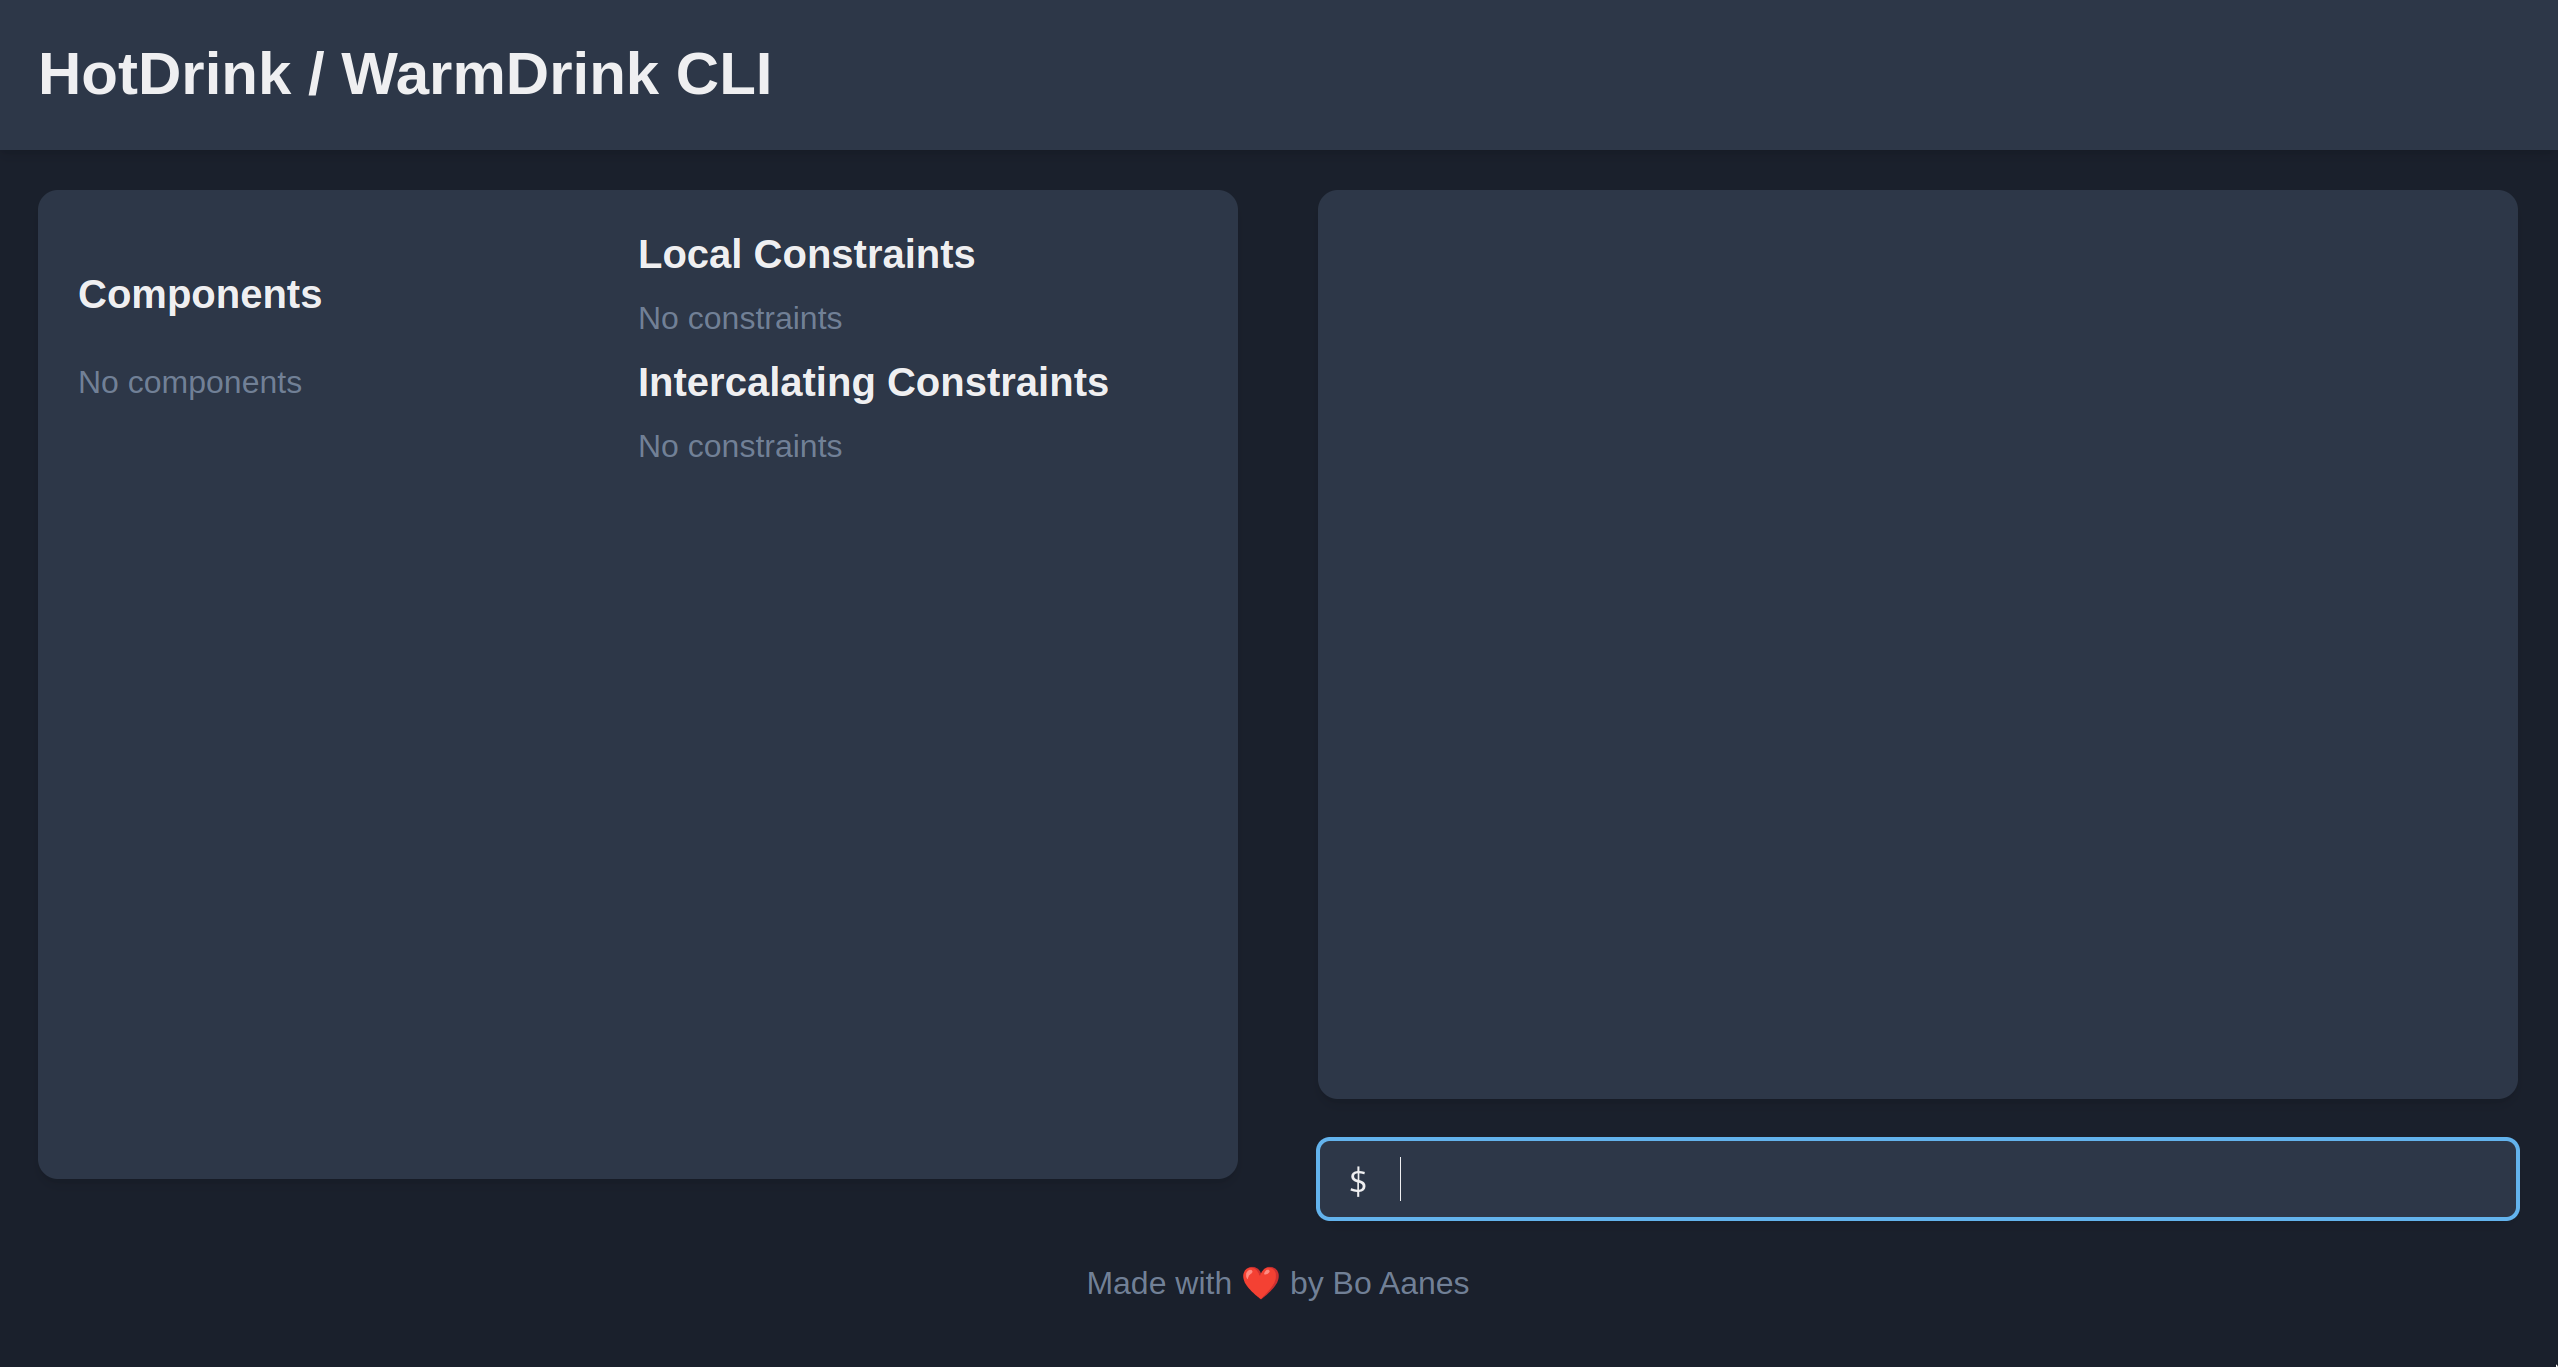
\includegraphics[width=1.2\textwidth]{figures/view.png}}
    \caption{The view of the constraint system and the terminal.}
    \label{fig:view}
\end{figure}

In addition to the view of the program, the \texttt{App}-component also manages the state of the constraint system. We have defined types for components, constraints, methods, variables and component lists as can be seen in Listing \ref{lst:types}.

\begin{lstlisting}[float, language=java, caption={Types for constraint systems.}, label={lst:types}]
export interface Method {
  methodName: string;
  inputs: string[];
  expressions: Array<[string, string | undefined]>;
}

export interface Constraint {
  constraintName: string;
  methods: Method[];
}

export interface Variable {
  varID: string;
  varValue: number | boolean;
}

export interface IComponent {
  compID: number;
  variables: Variable[];
  strength: string[];
}

export interface ComponentList {
  components: IComponent[];
}
\end{lstlisting}

To manage state in React we use a \textit{hook} \cite{reacthooks} called \texttt{useState}. \texttt{useState} is a function that takes an optional default value state and returns an array consisting of two elements. The first being the current state, and the second begin a function to update the state.

\begin{lstlisting}[float, language=java, caption={Using \texttt{useState} to manage state.}, label={lst:usestate}]
  const [components, setComponents] = useState<IComponent[]>([]);
  const [constraints, setConstraints] = useState<Constraint[]>([]);
  const [intercalatingConstraints, setIntercalatingConstraints] = useState<
    Constraint[]
  >([]);
  const [highlighted, setHighlighted] = useState<string[]>([]);
  const [enforceFromIndex, setEnforceFromIndex] = useState<number>(0);
\end{lstlisting}

\clearpage
\bibliographystyle{plain}
\bibliography{generators/refs}

\end{document}
